% :Author: Stefan Kottwitz
% :Source: TeXblog - TikZ: shaded cube
%          http://texblog.net/latex-archive/graphics/tikz-cube-3d/
\documentclass[12pt]{article}

\usepackage[table,dvipsnames]{xcolor}

% fontspec needs XeLaTeXe
\usepackage{fontspec}
%\setmainfont{STIX-Regular}
%\setmainfont[Color=000000,Scale=4.3]{STIX-Bold}
%\setmainfont[Color=000000,Scale=4.3]{Rockwell}
%\setmainfont{Rough Draft}
%\setmainfont[Color=000000,Scale=4.5]{Eras Bold ITC}
%\setmathrm{STIXMath-Regular} %use this font for math
%\setmathrm[Color=000000,Scale=4.3]{Adobe Garamond Pro} %use this font for math
\setmainfont[Color=000000,Scale=5]{Arial}
%\setmainfont[Color=000000,Scale=4.3]{Lucida Bright}
%\setmainfont[Color=000000,Scale=4.3]{Latin Modern Math}
%\setmainfont[Color=000000,Scale=5]{APL385}  

%\newfontinstance\bigeras[Color=000000,Scale=10.0]{Eras Bold ITC}
%\setmainfont

\usepackage{tikz}
\usepackage{verbatim}

%\usepackage[active,tightpage]{preview}
%\PreviewEnvironment{tikzpicture}
%\setlength\PreviewBorder{5pt}%

% cube colors used to build RGB cube
\newcommand{\jodred}[1]{\textcolor{red}{#1}}
\newcommand{\jodblue}[1]{\textcolor{RoyalBlue}{#1}}
\newcommand{\jodgreen}[1]{\textcolor{PineGreen}{#1}}


\begin{comment}

:Title: Sudoku 3D cube
:Tags: 3D, Transformations

This example shows how to create an effective 3D effect using the ``slant`` transformation.
Shading has been added to enhance the 3D impression. Read more about this example over
at TeXblog_. 

.. _TeXblog: http://texblog.net/latex-archive/graphics/tikz-cube-3d/

:Author: Stefan Kottwitz
:Source: `TeXblog - TikZ: shaded cube`__

.. __: http://texblog.net/latex-archive/graphics/tikz-cube-3d/

\end{comment}

\usetikzlibrary{positioning}
\begin{document}
\Huge
\bf
\pagestyle{empty}
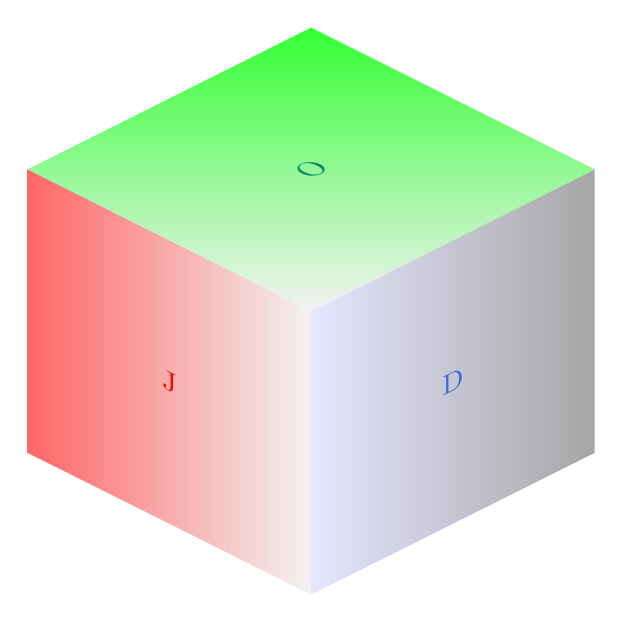
\begin{tikzpicture}[scale=1.2,every node/.style={minimum size=0in},on grid]
\begin{scope}[every node/.append style={yslant=-0.5},yslant=-0.5]
  \shade[right color=gray!10, left color=red!60] (0,0) rectangle +(3,3);
  \node at (1.5,1.5) {\jodred{J}};%{\includegraphics[height=1.0cm]{jred.png}};
%  \node at (1.5,2.5) {};
%  \node at (2.5,2.5) {};
%  \node at (0.5,1.5) {};
%  \node at (1.5,1.5) {O};%{\jodred{O}};
%  \node at (2.5,1.5) {};
%  \node at (0.5,0.5) {};
%  \node at (1.5,0.5) {};
%  \node at (2.5,0.5) {D};%{\textcolor{red}{D}};
%  \draw (0,0) grid (3,3);
\end{scope}
\begin{scope}[every node/.append style={yslant=0.5},yslant=0.5]
  \shade[right color=gray!70,left color=blue!10] (3,-3) rectangle +(3,3);
%  \node at (3.5,-0.5) {};
%  \node at (4.5,-0.5) {};
%  \node at (5.5,-0.5) {};
%  \node at (3.5,-1.5) {\includegraphics[height=1.0cm]{jblue.png}};
  \node at  (4.5,-1.5) {\jodblue{D}}; %{\textcolor{cyan}{O}}
%  \node at (5.5,-1.5) {D}; %{\textcolor{cyan}{D}}
%  \node at (3.5,-2.5) {};
%  \node at (4.5,-2.5) {};
%  \node at (5.5,-2.5) {};
%  \draw (3,-3) grid (6,0);
\end{scope}
\begin{scope}[every node/.append style={
    yslant=0.5,xslant=-1},yslant=0.5,xslant=-1
  ]
  \shade[bottom color=gray!10, top color=green!80] (6,3) rectangle +(-3,-3);
%  \node at (3.5,2.5) {};
%  \node at (3.5,1.5) {\includegraphics[height=1.0cm]{jgreen.png}}; 
%  \node at (3.5,0.5) {};
%  \node at (4.5,2.5) {};
 \node at (4.5,1.5) {\jodgreen{O}};%{\textcolor{ForestGreen}{O}}
%  \node at (4.5,0.5) {};
%  \node at (5.5,2.5) {};
%  \node at (5.5,1.5) {D};%{\textcolor{ForestGreen}{D}}
%  \node at (5.5,0.5) {};
%  \draw (3,0) grid (6,3);
\end{scope}
\end{tikzpicture}
\end{document}
